\documentclass[tikz]{standalone}
\usepackage{tikz}
\usetikzlibrary{calc,arrows,decorations.pathmorphing,backgrounds,positioning,fit,petri,shapes.misc,graphs}
\begin{document}
\tikzset{
    node distance=5mm,
    terminal/.style={
    % The shape:
    rounded rectangle,
    minimum size=6mm,
    % The rest
    very thick,draw=black!50,
    top color=white,bottom color=black!20,
    font=\ttfamily},
    nonterminal/.style={
    % The shape:
    rectangle,
    % The size:
    minimum size=6mm,
    % The border:
    very thick,
    draw=red!50!black!50, % 50% red and 50% black,
    % and that mixed with 50% white
    % The filling:
    top color=white, % a shading that is white at the top...
    bottom color=red!50!black!20, % and something else at the bottom
    % Font
    font=\itshape
    }
}
% 定义node风格
% nonterminals类型

\begin{tikzpicture}[
    nonterminal/.style={
    % The shape:
    rectangle,
    % The size:
    minimum size=6mm,
    % The border:
    very thick,
    draw=red!50!black!50, % 50% red and 50% black,
    % and that mixed with 50% white
    % The filling:
    top color=white, % a shading that is white at the top...
    bottom color=red!50!black!20, % and something else at the bottom
    % Font
    font=\itshape
    }]
    \node [nonterminal] {unsigned integer};
\end{tikzpicture}
% terminals类型,指定了使用圆角
% 刚好是minimu size的一半,所以单个字符时会是个圆

\begin{tikzpicture}[node distance=5mm,
    terminal/.style={
    % The shape:
    rectangle,minimum size=6mm,rounded corners=3mm,
    % The rest
    very thick,draw=black!50,
    top color=white,bottom color=black!20,
    font=\ttfamily}]
    \node (dot) [terminal] {.};
    \node (digit) [terminal,right=of dot] {digit};
    \node (E) [terminal,right=of digit] {E};
\end{tikzpicture}
% 使用shapes.misc中提供的rounded rectangle也能达到
% 要求,而且这个包还提供了更灵活的功能

\begin{tikzpicture}[node distance=5mm,
    terminal/.style={
    % The shape:
    rounded rectangle,
    minimum size=6mm,
    % The rest
    very thick,draw=black!50,
    top color=white,bottom color=black!20,
    font=\ttfamily}]
    \node (dot) [terminal] {.};
    \node (digit) [terminal,right=of dot] {digit};
    \node (E) [terminal,right=of digit] {E};
\end{tikzpicture}
% 画基线,作对比,发现几个node的基线没有对齐
\begin{tikzpicture}[node distance=5mm]
    \node (dot) [terminal] {.};
    \node (digit) [terminal,right=of dot] {digit};
    \node (E) [terminal,right=of digit] {E};
    \draw [help lines] let \p1 = (dot.base),
    \p2 = (digit.base),
    \p3 = (E.base)
    in (-.5,\y1) -- (3.5,\y1)
    (-.5,\y2) -- (3.5,\y2)
    (-.5,\y3) -- (3.5,\y3);
\end{tikzpicture}
% 想当然的对齐方案,用base right代替right
\begin{tikzpicture}[node distance=5mm]
    \node (dot) [terminal] {.};
    \node (digit) [terminal,base right=of dot] {digit};
    \node (E) [terminal,base right=of digit] {E};
\end{tikzpicture}
% right和base right的差别
% 关于right=of X的含义,就是当前node自己的
% west anchor位于X的east anchor的右边多少多少
% 而加了base之后则是底部的对应方向的anchor的
% 偏移关系。总体而言是两个node的相向的anchor
% 的偏移关系,而不是固定的anchor的偏移关系,
% 这点可以通过更改node里文字长度来测试出来,
% 实际效果是,文字长度变了,node间距依然没变。
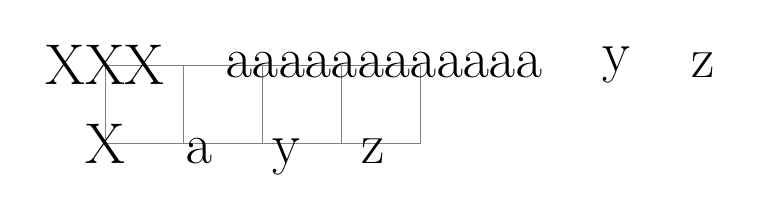
\begin{tikzpicture}[node distance=1ex]
    \draw[help lines] (0,0) grid (4,1);
    \huge
    \node (X) at (0,1) {XXX};
    \node (a) [right=of X] {aaaaaaaaaaaa};
    \node (y) [right=of a] {y};
    \node (z) [right=of y] {z};
    \node (X) at (0,0) {X};
    \node (a) [base right=of X] {a};
    \node (y) [base right=of a] {y};
    \node (z) [base right=of y] {z};
\end{tikzpicture}
% 最终解决方案是为文字指定相同的高度和深度(不知道是啥)
% 这样之后,文字基线也一致了,node也不乱跑了
\begin{tikzpicture}[node distance=5mm,
    text height=1.5ex,text depth=.25ex]
    \node (dot) [terminal] {.};
    \node (digit) [terminal,right=of dot] {digit};
    \node (E) [terminal,right=of digit] {E};
\end{tikzpicture}

% 手动对齐的不足之处有:
% 1.对复杂图形,坐标很难计算;
% 2.一旦文字内容改变,坐标需要重新计算
% 3.节点间相对关系不明确,源码可读性差
% 使用位置选项对node进行对齐
% 这种方式下E和+号其实水平方向上很近,和预想的不一致
% 原因是,当指定+号在E的右上方时,是说+号的西南锚点
% 在E的东北锚点的右上方,rounded rectangle会影响锚点位置,
% +号的西南锚点是正下方位置,E的东北锚点也是正上方位置,
% 这两个位置按规则对齐导致,实际节点没按规则对齐。
\begin{tikzpicture}[node distance=5mm and 5mm]
    \node (ui1) [nonterminal] {unsigned integer};
    \node (dot) [terminal,right=of ui1] {.};
    \node (digit) [terminal,right=of dot] {digit};
    \node (E) [terminal,right=of digit] {E};
    \node (plus) [terminal,above right=of E] {+};
    \node (minus) [terminal,below right=of E] {-};
    \node (ui2) [nonterminal,below right=of plus] {unsigned integer};
\end{tikzpicture}
% 一种解决方法是手动多添加一些水平位移
\begin{tikzpicture}[node distance=5mm and 5mm]
    \node (E) [terminal] {E};
    \node (plus) [terminal,above right=of E,xshift=5mm] {+};
    \node (minus) [terminal,below right=of E,xshift=5mm] {-};
    \node (ui2) [nonterminal,below right=of plus,xshift=5mm] {unsigned integer};
\end{tikzpicture}
% 另一种解决方法是terminal不再使用rounded rectangle,而是使用
% 普通的rectangle然后用圆角选项,圆角选项不影响锚点的位置,因此
% 能得到正确的结果
\begin{tikzpicture}[node distance=5mm and 5mm,terminal/.append style={rectangle,rounded corners=3mm}]
    \node (E) [terminal] {E};
    \node (plus) [terminal,above right=of E] {+};
    \node (minus) [terminal,below right=of E] {-};
    \node (ui2) [nonterminal,below right=of plus] {unsigned integer};
\end{tikzpicture}
% 第三种方法是用矩阵后面再说

% 画直角拐弯的连接线,而且有锚点和向量做线性组合的例子
\begin{tikzpicture}[node distance=5mm and 5mm]
    \node (dot) [terminal] {.};
    \node (digit) [terminal,right=of dot] {digit};
    \node (E) [terminal,right=of digit] {E};
    \path (dot) edge[->] (digit) % simple edges
    (digit) edge[->] (E);
    \draw [->]
    % start right of digit.east, that is, at the point that is the
    % linear combination of digit.east and the vector (2mm,0pt). We
    % use the ($ ... $) notation for computing linear combinations
    ($ (digit.east) + (2mm,0) $)
    % Now go down
    -- ++(0,-.5)
    % And back to the left of digit.west
    -| ($ (digit.west) - (2mm,0) $);
\end{tikzpicture}
% 使用edge,关于edge的详细机制暂时先不深究
% 文档中写道: Whenever the edge command is used, 
% it simply adds the current value of "to path" to the path. 
% So, Ilka can set up a style that contains the correct path
% 文档159页有关于to path的解释待进一步测试
% 除了to path的机制之外,这个例子中还有连接线的常用符号
% -|和|-,分别表示先水平后垂直和先垂直后水平的连接线
% \tikztotarget是个宏,会展开为特定的点
\begin{tikzpicture}[node distance=5mm and 5mm,
    skip loop/.style={to path={-- ++(0,-.5) -| (\tikztotarget)}}]
    \node (dot) [terminal] {.};
    \node (digit) [terminal,right=of dot] {digit};
    \node (E) [terminal,right=of digit] {E};
    \path (dot) edge[->] (digit) % simple edges
    (digit) edge[->] (E)
    ($ (digit.east) + (2mm,0) $)
    edge[->,skip loop] ($ (digit.west) - (2mm,0) $);
\end{tikzpicture}
% 上面例子中偏移量可以参数化,线性组合的方式也有所变化
\begin{tikzpicture}[node distance=5mm and 5mm,
    skip loop/.style={to path={-- ++(0,#1) -| (\tikztotarget)}}]
    \node (dot) [terminal] {.};
    \node (digit) [terminal,right=of dot] {digit};
    \node (E) [terminal,right=of digit] {E};
    \path (dot) edge[->] (digit) % simple edges
    (digit) edge[->] (E)
    ($ (digit.east)!.5!(E.west) $)
    edge[->,skip loop=-5mm] ($ (digit.west)!.5!(dot.east) $);
\end{tikzpicture}
% 使用矩阵对齐node,使用latex中的&来换列,\\来换行
% 这部分只是改进了上面那些例子的\node部分的内容,
% 连接线的绘制还是照旧
\begin{tikzpicture}
    \matrix[row sep=1mm,column sep=5mm] {
    % First row:
    & & & & \node [terminal] {+}; & \\
    % Second row:
    \node [nonterminal] {unsigned integer}; &
    \node [terminal] {.}; &
    \node [terminal] {digit}; &
    \node [terminal] {E}; &
    &
    \node [nonterminal] {unsigned integer}; \\
    % Third row:
    & & & & \node [terminal] {-}; & \\
    };
\end{tikzpicture}
% 更进一步,在用矩阵布局时可以放入一些固定点node
% 在后面绘制连接线时就可以直接连这些node了,而不再需要
% 指定线性组合坐标
\begin{tikzpicture}[point/.style={circle,inner sep=0pt,minimum size=2pt,fill=red},
    skip loop/.style={to path={-- ++(0,#1) -| (\tikztotarget)}}]
    \matrix[row sep=1mm,column sep=2mm] {
    % First row:
    & & & & & & & & & & & \node (plus) [terminal] {+};\\
    % Second row:
    \node (p1) [point] {}; & \node (ui1) [nonterminal] {unsigned integer}; &
    \node (p2) [point] {}; & \node (dot) [terminal] {.}; &
    \node (p3) [point] {}; & \node (digit) [terminal] {digit}; &
    \node (p4) [point] {}; & \node (p5) [point] {}; &
    \node (p6) [point] {}; & \node (e) [terminal] {E}; &
    \node (p7) [point] {}; & &
    \node (p8) [point] {}; & \node (ui2) [nonterminal] {unsigned integer}; &
    \node (p9) [point] {}; & \node (p10) [point] {};\\
    % Third row:
    & & & & & & & & & & & \node (minus)[terminal] {-};\\
    };
    \path (p4) edge [->,skip loop=-5mm] (p3)
    (p2) edge [->,skip loop=5mm] (p6);
\end{tikzpicture}
% 上面使用矩阵的方式做对齐已经得到很好地效果,而连接node
% 还有一个比edge更好的方案,就是使用graph库
% graph既能连接已有的node,也能临时创建新node
\begin{tikzpicture}[
    skip loop/.style={to path={-- ++(0,#1) -| (\tikztotarget)}},
    hv path/.style={to path={-| (\tikztotarget)}},
    vh path/.style={to path={|- (\tikztotarget)}},
    point/.style={circle,inner sep=0pt,minimum size=2pt,fill=red}]
    \matrix[row sep=1mm,column sep=2mm] {
    % First row:
    & & & & & & & & & & & \node (plus) [terminal] {+};\\
    % Second row:
    \node (p1) [point] {}; & \node (ui1) [nonterminal] {unsigned integer}; &
    \node (p2) [point] {}; & \node (dot) [terminal] {.}; &
    \node (p3) [point] {}; & \node (digit) [terminal] {digit}; &
    \node (p4) [point] {}; & \node (p5) [point] {}; &
    \node (p6) [point] {}; & \node (e) [terminal] {E}; &
    \node (p7) [point] {}; & &
    \node (p8) [point] {}; & \node (ui2) [nonterminal] {unsigned integer}; &
    \node (p9) [point] {}; & \node (p10) [point] {};\\
    % Third row:
    & & & & & & & & & & & \node (minus)[terminal] {-};\\
    };
    \graph {
    (p1) -> (ui1) -- (p2) -> (dot) -- (p3) -> (digit) -- (p4)
    -- (p5) -- (p6) -> (e) -- (p7) -- (p8) -> (ui2) -- (p9) -> (p10);
    (p4) ->[skip loop=-5mm] (p3);
    (p2) ->[skip loop=5mm] (p5);
    (p6) ->[skip loop=-11mm] (p9);
    (p7) ->[vh path] (plus) -> [hv path] (p8);
    (p7) ->[vh path] (minus) -> [hv path] (p8);
    };
\end{tikzpicture}
% 进一步简化,使用use existing nodes选项,对node的引用可以免去
% 括号了,而且能够用一个node连接一组node的方式简化E到+号和-号的
% 连接,总体而言,代码更清晰
\begin{tikzpicture}[,thick,black!50,text=black,
    every new ->/.style={shorten >=1pt},
    graphs/every graph/.style={edges=rounded corners},
    skip loop/.style={to path={-- ++(0,#1) -| (\tikztotarget)}},
    hv path/.style={to path={-| (\tikztotarget)}},
    vh path/.style={to path={|- (\tikztotarget)}},
    point/.style={circle,inner sep=0pt,minimum size=2pt,fill=red}]
    \matrix[row sep=1mm,column sep=2mm] {
    % First row:
    & & & & & & & & & & & \node (plus) [terminal] {+};\\
    % Second row:
    \node (p1) [point] {}; & \node (ui1) [nonterminal] {unsigned integer}; &
    \node (p2) [point] {}; & \node (dot) [terminal] {.}; &
    \node (p3) [point] {}; & \node (digit) [terminal] {digit}; &
    \node (p4) [point] {}; & \node (p5) [point] {}; &
    \node (p6) [point] {}; & \node (e) [terminal] {E}; &
    \node (p7) [point] {}; & &
    \node (p8) [point] {}; & \node (ui2) [nonterminal] {unsigned integer}; &
    \node (p9) [point] {}; & \node (p10) [point] {};\\
    % Third row:
    & & & & & & & & & & & \node (minus)[terminal] {-};\\
    };
    \graph [use existing nodes] {
    p1 -> ui1 -- p2 -> dot -- p3 -> digit -- p4 -- p5 -- p6 -> e -- p7 -- p8 -> ui2 -- p9 -> p10;
    p4 ->[skip loop=-5mm] p3;
    p2 ->[skip loop=5mm] p5;
    p6 ->[skip loop=-11mm] p9;
    p7 ->[vh path] { plus, minus } -> [hv path] p8;
    };
\end{tikzpicture}
% 使用graph创建node,当没有使用use existing nodes选项,且用名字
% 引用node没加括号时,tikz就会创建一个名字和文本都是这个名字的node
% 其他node名可以直接用字符串,点号得用引号括起来
% grow right sep指定了graph往那边扩展
\begin{tikzpicture}
    \graph[grow right sep]
    {first node[nonterminal] -> "."[terminal] -> second node[terminal] -> last node[terminal]};
\end{tikzpicture}
% 使用一个node到一组node的连接,同时新建一个node显示相同的文本,
% 如果这里直接用同一个文本,tikz会把它识别成已有的node,所以连接
% 会指回到前面的node,因此需要用name/text的形式创建一个新node,
% 如果这个node在后面不会再被引用,那可以创建一个不具名的node,省略掉
% node名直接用 /text的形式创建,这样始终表示一个新建的、不具名的节点。
\begin{tikzpicture}
    \graph [grow right sep] {
        unsigned integer [nonterminal] ->
        "." [terminal] ->
        digit [terminal] ->
        E [terminal] ->
        {
        "+" [terminal],
        "" [coordinate],
        "-" [terminal]
        } ->
        ui2/unsigned integer [nonterminal]
        };
\end{tikzpicture}
% 下面的例子在E分叉处的结果比较奇怪
% 原因在于E往+号和-号应该用-|,但是往
% q2应该直接用水平线过去,但是这里还是强制用了拐线
% 而且这里q2起到占位作用,影响了布局,如果把q2去掉,就不是一个
% 上中下的结构了,-号会跟q1一个水平,那拐线还是不对
\begin{tikzpicture}[thick, black!50, text=black,
    every new ->/.style={shorten >=1pt},
    graphs/every graph/.style={edges=rounded corners},
    skip loop/.style={to path={-- ++(0,#1) -| (\tikztotarget)}},
    hv path/.style={to path={-| (\tikztotarget)}},
    vh path/.style={to path={|- (\tikztotarget)}}]
    \graph [grow right sep, branch down=7mm] {
    / [coordinate] ->
    unsigned integer [nonterminal] --
    p1 [coordinate] ->
    "." [terminal] --
    p2 [coordinate] ->
    digit [terminal] --
    p3 [coordinate] --
    p4 [coordinate] --
    p5 [coordinate] ->
    E [terminal] --
    q1 [coordinate] ->[vh path]
    { [nodes={yshift=7mm}]
    "+" [terminal],
    q2/ [coordinate],
    "-" [terminal]
    } -> [hv path]
    q3 [coordinate] --
    /unsigned integer [nonterminal] --
    p6 [coordinate] ->
    / [coordinate];
    p1 ->[skip loop=5mm] p4;
    p3 ->[skip loop=-5mm] p2;
    p5 ->[skip loop=-11mm] p6;
    };
\end{tikzpicture}
% 一个解决上面问题的方法,是使用graph的simple选项,开启之后
% 每两个node之间最多只能有一个连接,那么如果一个连接指定两次,
% 后面的设置会覆盖前面的设置。因此可以在graph的最后再设置一遍
% q1到q2到q3的直线连接,覆盖掉前面的拐弯连接线
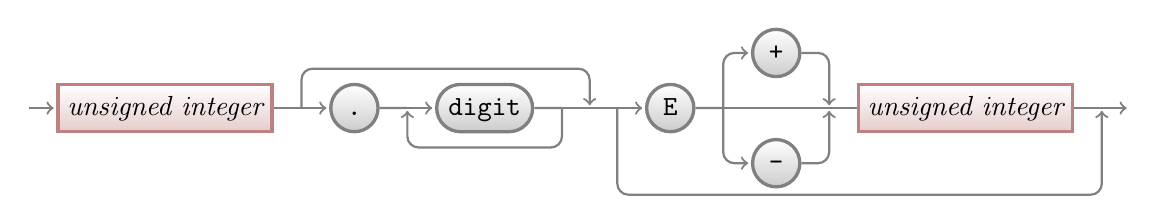
\begin{tikzpicture}
[black!50, text=black, thick,
every new ->/.style = {shorten >=1pt},
graphs/every graph/.style = {edges=rounded corners},
skip loop/.style = {to path={-- ++(0,#1) -| (\tikztotarget)}},
hv path/.style = {to path={-| (\tikztotarget)}},
vh path/.style = {to path={|- (\tikztotarget)}},
nonterminal/.style = {rectangle, minimum size=6mm, very thick, draw=red!50!black!50, top color=white,
                      bottom color=red!50!black!20, font=\itshape, text height=1.5ex,text depth=.25ex},
terminal/.style = {rounded rectangle, minimum size=6mm, very thick, draw=black!50, top color=white,
                   bottom color=black!20, font=\ttfamily, text height=1.5ex, text depth=.25ex},
shape = coordinate]
\graph [grow right sep, branch down=7mm, simple] {
/ -> unsigned integer[nonterminal] -- p1 -> "." [terminal] -- p2 -> digit[terminal] --
p3 -- p4 -- p5 -> E[terminal] -- q1 ->[vh path]
{[nodes={yshift=7mm}]
"+"[terminal], q2, "-"[terminal]
} -> [hv path]
q3 -- /unsigned integer [nonterminal] -- p6 -> /;
p1 ->[skip loop=5mm] p4;
p3 ->[skip loop=-5mm] p2;
p5 ->[skip loop=-11mm] p6;
q1 -- q2 -- q3; % make these edges plain
};
\end{tikzpicture}
\end{document}